\documentclass[a4paper,12pt]{report}

\usepackage{alltt, fancyvrb, url}
\usepackage{graphicx}
\usepackage[utf8]{inputenc}
\usepackage{float}
\usepackage{hyperref}
\usepackage[italian]{babel}
\usepackage{appendix}
\usepackage[italian]{cleveref}
\usepackage{xcolor}
\usepackage{microtype}
\usepackage{array}
\usepackage{adjustbox}
\usepackage{tabularx}
\usepackage{colortbl}
\usepackage{pdfpages}
\usepackage{listings}

\lstdefinestyle{codeStyle}{
    basicstyle=\small\ttfamily,
    keywordstyle=\color{blue},
    commentstyle=\color{green},
    stringstyle=\color{red},
    numbers=left,
    numberstyle=\tiny\color{gray},
    frame=single,
    breaklines=true,
    tabsize=4
}
\lstset{}





\graphicspath{{./resources/img}}
\title{Elaborato Basi di Dati}
\author{Desiderio Edoardo}
\begin{document}
\maketitle
\titlepage
\tableofcontents
\newpage

\chapter{Analisi dei requisiti}
Lo scopo è realizzare un portale che permetta alla società richiedente di gestire in maniera informatizzata le prenotazini e l'organizzazione
delle visite guidate che vuole organizzare con i siti di maggior interesse.
\section{Intervista}
Una	 società	 operante	 nel	 settore	 del	 turismo	 offre	 tra	 i	 suoi	 servizi	 l’organizzazione	 di	 	 visite
guidate	a	siti	d' interesse	storico-culturale.
Ogni	visita,	opportunamente	descritta,	ha	un	 titolo	 (diverse	visite	hanno	un	 titolo	 ricorrente,	es.
“Musei	Vaticani	e	Cappella	Sistina”,	“Sito	archeologico	di	Pompei”,	“Galleria	degli	uffizi”,	ecc.),	la
sua	durata	media		e	il	luogo		in	cui	essa	si	svolge.	Ogni	visita	può	avere	luogo	più	volte	nel	tempo
secondo	specifici	eventi	programmati.
Le escursioni,	di	cui	viene	indicato	il	prezzo,	vengono	prenotati	da	gruppi	di	persone	condotti	da	una
guida	che	illustra	il	percorso	in	una	determinata	lingua;	per	ogni	gruppo	viene	fissata	l’ora	d' inizio
della	visita	e un	numero	minimo	e	massimo	di	partecipanti.
Il prezzo degli eventi varia in base all'età:
\begin{itemize}
	\item 0-12 il prezzo è gratuito
	\item 12-14 il prezzo è scontato del 20\%
	\item gli over 50 godono di uno sconto pari al 10\%
\end{itemize}
La	società	si	avvale	di	diverse	guide	ognuna	delle	quali	ha	competenze	in	una	o	più	lingue	ad uno
specifico	 livello	 di	 conoscenza	 ("B2","C1","C2"). Di ogni capo gruppo	 si	 vuole
conoscere	 alcuni	 dati	 tra	 i	 quali	 nome,	 sesso,	 data	 di	 nascita,	 titolo	 di	 studio	 e	 relativo	 anno	 di
conseguimento.
\\
I	clienti,	di	cui	si	vuole	conoscere	almeno	nome,	nazionalità,	lingua	base,	e-mail	e	un	 recapito
telefonico,	 possono	 aggregarsi	 a	 uno	 o	 più	 gruppi,	 secondo	 le	 loro	 esigenze.	 Uno	 stesso
visitatore,	 nel	 tempo,	 può	 partecipare	 a	 gruppi	 diversi	 usando	 ogni	 volta	 una	 certa	 forma	 di
pagamento	(non	necessariamente	sempre	la	stessa	es.	Carta	di	credito,	paypal,	bonifico	bancario)
della	quale	si	deve	prevedere	la	memorizzazione:	tipologia,	descrizione	e	data	del	pagamento.
Il	 sito	 web	 della	 società	 consente	 la	 visione	 pubblica	 delle	 visite	 organizzate	 e,	 solo	 agli	 utenti
preventivamente	registrati,	la	prenotazione	di	una	specifica	visita. In fine l'applicativo
deve permettere una visione protetta dei dati, quindi non tutti gli utenti ad esempio possono
visionare i gruppi a cui sono affidate le guide

\section{Rilevamento delle ambiguità e correzioni proposte}
Il testo dell'intervista presenta molte ambiguità. Le principali sono
\begin{itemize}
	\item utilizzo di sinonimi
	\item Elenchi di attributi incompleti
	\item Cartdinalità non specificate
\end{itemize}

Gli attributi parziali e le cardinalità verranno risolti mediante l'uso della logica in fase di creazione dello schema concettuale.
Invece per quanto concerne i sinonimi, è necessario costruire un glossario dei termini


\begin{table}[H]
	\begin{center}
		\begin{tabularx}{\textwidth}{|>{\centering\arraybackslash}X|>{\centering\arraybackslash}X|>{\centering\arraybackslash}X|>{\centering\arraybackslash}X|}
			\hline
			\rowcolor{red} termine & descrizione                                                                & sinonimi                   & collegamenti                                     \\
			\hline
			utente                 & entità che interagisce con il database lato consumatore                    & cliente, visitatore        & gruppi, pagamenti, sconti                        \\
			\hline
			guida                  & figura qualificata in lingue e storia che illustra il percorso passo passo & capo gruppo, dipendente    & turni di lavoro, competenze linguistiche, gruppi \\
			\hline
			sconto                 & rappresenta la percentuale da decurtare al prezzo finale in base all'età   & -                          & pagamento, cliente                               \\
			\hline
			gruppo                 & insieme di persone in questo caso                                          & -                          & cliente, guida, evento                           \\
			\hline
			evento                 & situazione specifica dato un luogo e orario                                & visita-guidata, escursioni & visita, gruppi                                   \\
			\hline
			visite                 & logo d'interesse con cui ha accordi la società di turismo                  & sito culturale             & eventi                                           \\
			\hline
		\end{tabularx}
		\caption{\label{glossario:termini}} termini rappresentativi dell' intervista
	\end{center}
\end{table}


\subsection*{Ipotesi aggiuntive}
dall'intervista fatta si concretizza che:
\begin{itemize}
	\item il dato relativo alla durata media di una visita venga espresso in minuti
	\item  per	uno	specifico	evento	di	visita	guidata	possano	essere	formati	anche	più	gruppi		ognuno
	      col	proprio	orario,	accompagnatore	e	lingua;
	\item i	 vari	 visitatori	 per	 potersi	 iscriversi	 ad	 uno	 o	 più	 eventi	 debbono	 registrarsi	 sul	 sito	 della
	      società	 fornendo	 e-mail	 e	 password.	 La	 banca	 dati	 non	 prevede	 alcuna	 gestione
	      relativamente	 agli	 utenti	 anonimi:	 essi	 possono	 operare	 solo	 per	 funzionalità	 limitate	 d'
	      interrogazione	per	vedere	i	dati	degli	eventi	programmati;
	\item per	potersi	iscrivere	ad	un	gruppo	di	visita	relativamente	ad	uno	specifico	evento,	nei	limiti
	      della	 disponibilità	 di	 posti,	 ogni	 visitatore	 registrato	 effettui	 il	 pagamento	 tramite	 carta	 di
	      credito	 (con	 codice	 della	 medesima),	 via	 PayPal	 (l’utente	 deve	 essere	 registrato	 a	 tale
	      servizio),	 o	 tramite	 bonifico	 bancario	 di	 cui	 deve	 fornire	 gli	 estremi	 utilizzando	 il	 campo
	      relativo	alla	descrizione	del	pagamento;
	\item il	prezzo	di	una	visita	sia	comunque	individuale	e	venga	espresso	a	livello	di	evento	in	quanto
	      suscettibile	di	variazioni	nel	tempo
	\item per definire `gratuito' il prezzo di un biglietto si imposterà una percentuale di sconto pari al 100\%
\end{itemize}


\newpage
\section{Definizione delle specifiche in linguaggio naturale ed estrazione dei concetti principali}
Di seguito si riporta un testo riassuntivo in cui sono evidenziati i concetti chiave
dell’ intervista filtrati dalle ambiguità possibili, in modo da avere un’ idea più chiara di
quelle che saranno le entità presenti nello schema concettuale.\\\\
La società commissionatrice vuole creare la gestione informatizzata dei suoi servizi.\\
Ogni \textbf{\underline{visita}}, intesa come il sito culturale è opportunamente descritta definendo
il titolo, luogo, identificativo, descrizione, durata media espressa in minuti.\\
Per ogni visita la società organizza degli eventi. Ogni \textbf{\underline{evento}} può ripetersi più volte
rispetto ad una determinata visita e ne viene definito il prezzo indicato che può variare nel tempo; si vuole memorizzare anche
la data dell'evento.\\\\
I \textbf{\underline{clienti}}, di cui si salvano lingua preferenza e dati principali una password e mail per accedere a funzionalità
più avanzate per la prenotazione di biglietti ecc, vengono assegnati a gruppi differenti in base alle loro preferenze
proposte  al momento dell'acquisto dei \textbf{biglietti}. Per gestire i pagamenti il cliente potrà aggiungere al carrello i biglietti che intende
acquistare per poi procedere al pagamento utilizzando quello che più preferisce (paypall, bonifico, carta di credito) \\\\
Dei \textbf{\underline{Gruppi}} si vuole indicare l'orario d' inizio della visita si vuole specificare
il minimo numero di persone da cui deve essere composto un gruppo e il massimo, bisogna valutare
se è conveniente salvare anche il numero d' iscritti correnti o lasciare il dato deducibile.\\\\
I \textbf{\underline{biglietti}} devono essere acquistati dall'utente, siccome ogni utente può acquistare biglietti anche per altre persone
ogni biglietto deve specificare il nome e il cognome e l'età della persona per cui
viene acquistato il biglietto siccome sono previste fasce di \textbf{\underline{sconto}} in base all'età.
Rispettivamente \(eta \le 12 \rightarrow\)  100\%, \(12 < eta \le 14 \rightarrow\)  20\%, \(eta >50 \rightarrow\)  10\%.
Per ogni nuovo evento vengono emessi biglietti pari al numero minimo di partecipanti di un gruppo\\\\
IL \textbf{\underline{carrello}} deve raccogliere le registrazioni per biglietti a persona per poi calcolare
il totale dell'ordine. A livello applicativo sarà gestito da una vista che assocerà gli ordini fatti dal cliente \\\\
Delle \textbf{\underline{guide}} turistiche oltre ai dati comuni con il cliente si vuole memorizzare
anche il titolo di studio e il suo anno di conseguimento. La società intende registrare i dati relativi
alle \textbf{\underline{competenze}}. Ogni competenza deve essere riferita ad una guida e alle lingue che essa conosce,
il livello di conoscenza deve essere espresso in (B2,C1,C2).

\section*{Individuazione operazioni principali}
\begin{itemize}
	\item Aggiunta di eventi per ogni tipo di visite
	\item inserimento di un nuovo cliente
	\item inserimento di una nuova guida
	\item gestione e riepilogo ordini
	\item Aggiunta di un nuovo gruppo
	\item creazione di biglietti fino al numero minimo di partecipanti ad un gruppo
	\item vendita di biglietti per un determinato cliente
	\item applicazione sconto in base al destinatario del biglietto acquistato
	\item storico degli acquisti
	\item controllo del riempimento dei gruppi
	\item assegnazione di una determinata guida ad un gruppo in base alle sue conoscenze
	\item indicazione dei posti rimanenti per le iscrizioni ad un gruppo
\end{itemize}

\newpage
\chapter{Progettazione concettuale}
Per maggiore chiarezza, di seguito riportiamo i primi esempi di schemi concettuali
divisi per ambiti. Partirò da parti di schema concettuale più semplici fino ad arrivare a parti più complesse
\subsection*{Visita-Evento-Gruppo}
\begin{figure}[H]
	\centering
	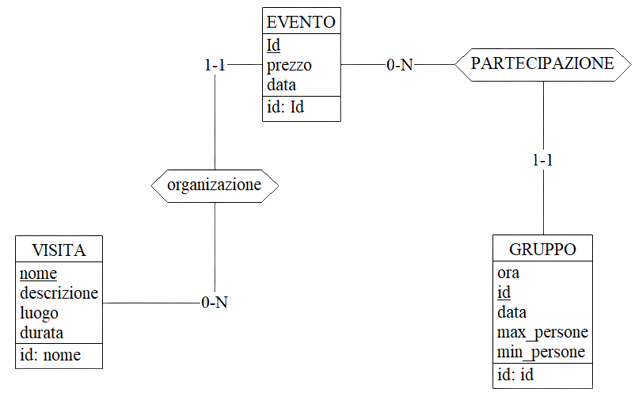
\includegraphics[width=0.99\textwidth]{evento-visita-gruppo.png}
	\caption[]{caratterizzazione della gestione fra le visite, i vari eventi che può ospitare e i gruppi che vi partecipano}
\end{figure}
Lo schema è piuttosto auto esplicativo, sono stati mantenuti i vincoli imposti
dall'intervista come permettere l'Associazione di più eventi data una visita e 
la partecipazione di più gruppi al determinato evento si noti come da un gruppo 
si possa risalire ad un determinato evento e ad una determinata visita.
\subsection*{Gerarchia persone, relazione fra gruppi guide e competenze}
\begin{figure}[H]
	\centering
	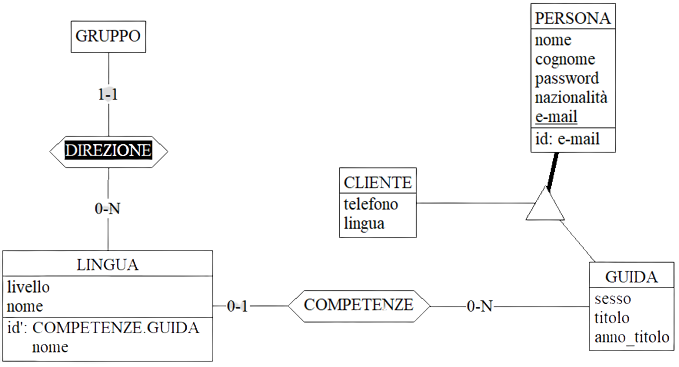
\includegraphics[width=0.99\textwidth]{gruppo-guide.png}
	\caption[]{l'entità gruppo è descritta nella figura sopra}
\end{figure}

Per gestire le entità CLIENTE, GUIDA poiché ave\-vano campi
simili ho optato per una gerar\-chia di tipo totale ed Esclusiva 
( DB\_MAIN non mostrava la scritta t, e)\-.
Il resto dello schema E-R portato esplicita la modellazione di associare 
più tipi di lingue ad una determinata guida. Lingua quindi è un'entità debole
che necessita della chiave di GUIDA per essere completa. Adottando questo metodo
per ogni gurppo posso risalire alla guida e con che lingua e a che livello sarà
diretto.

\subsection*{Biglietto-Ordine-Cliente}

\begin{figure}[H]
	\centering
	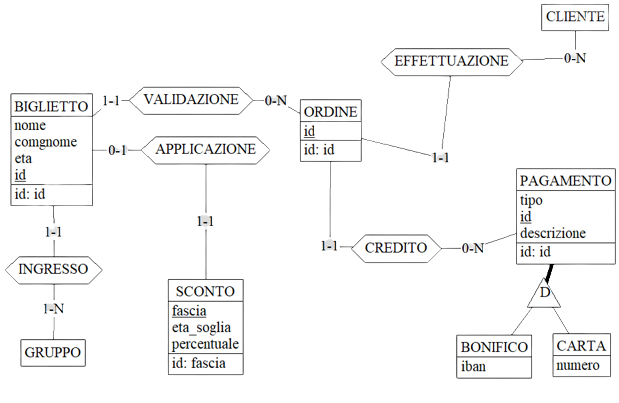
\includegraphics[width=0.99\textwidth]{BIGLIETTO-ORDINE.png}
	\caption{i biglietti rappresentano il punto di collegamento relazionale fra i gruppi e i clienti}
\end{figure}



\section{Schema scheletro}

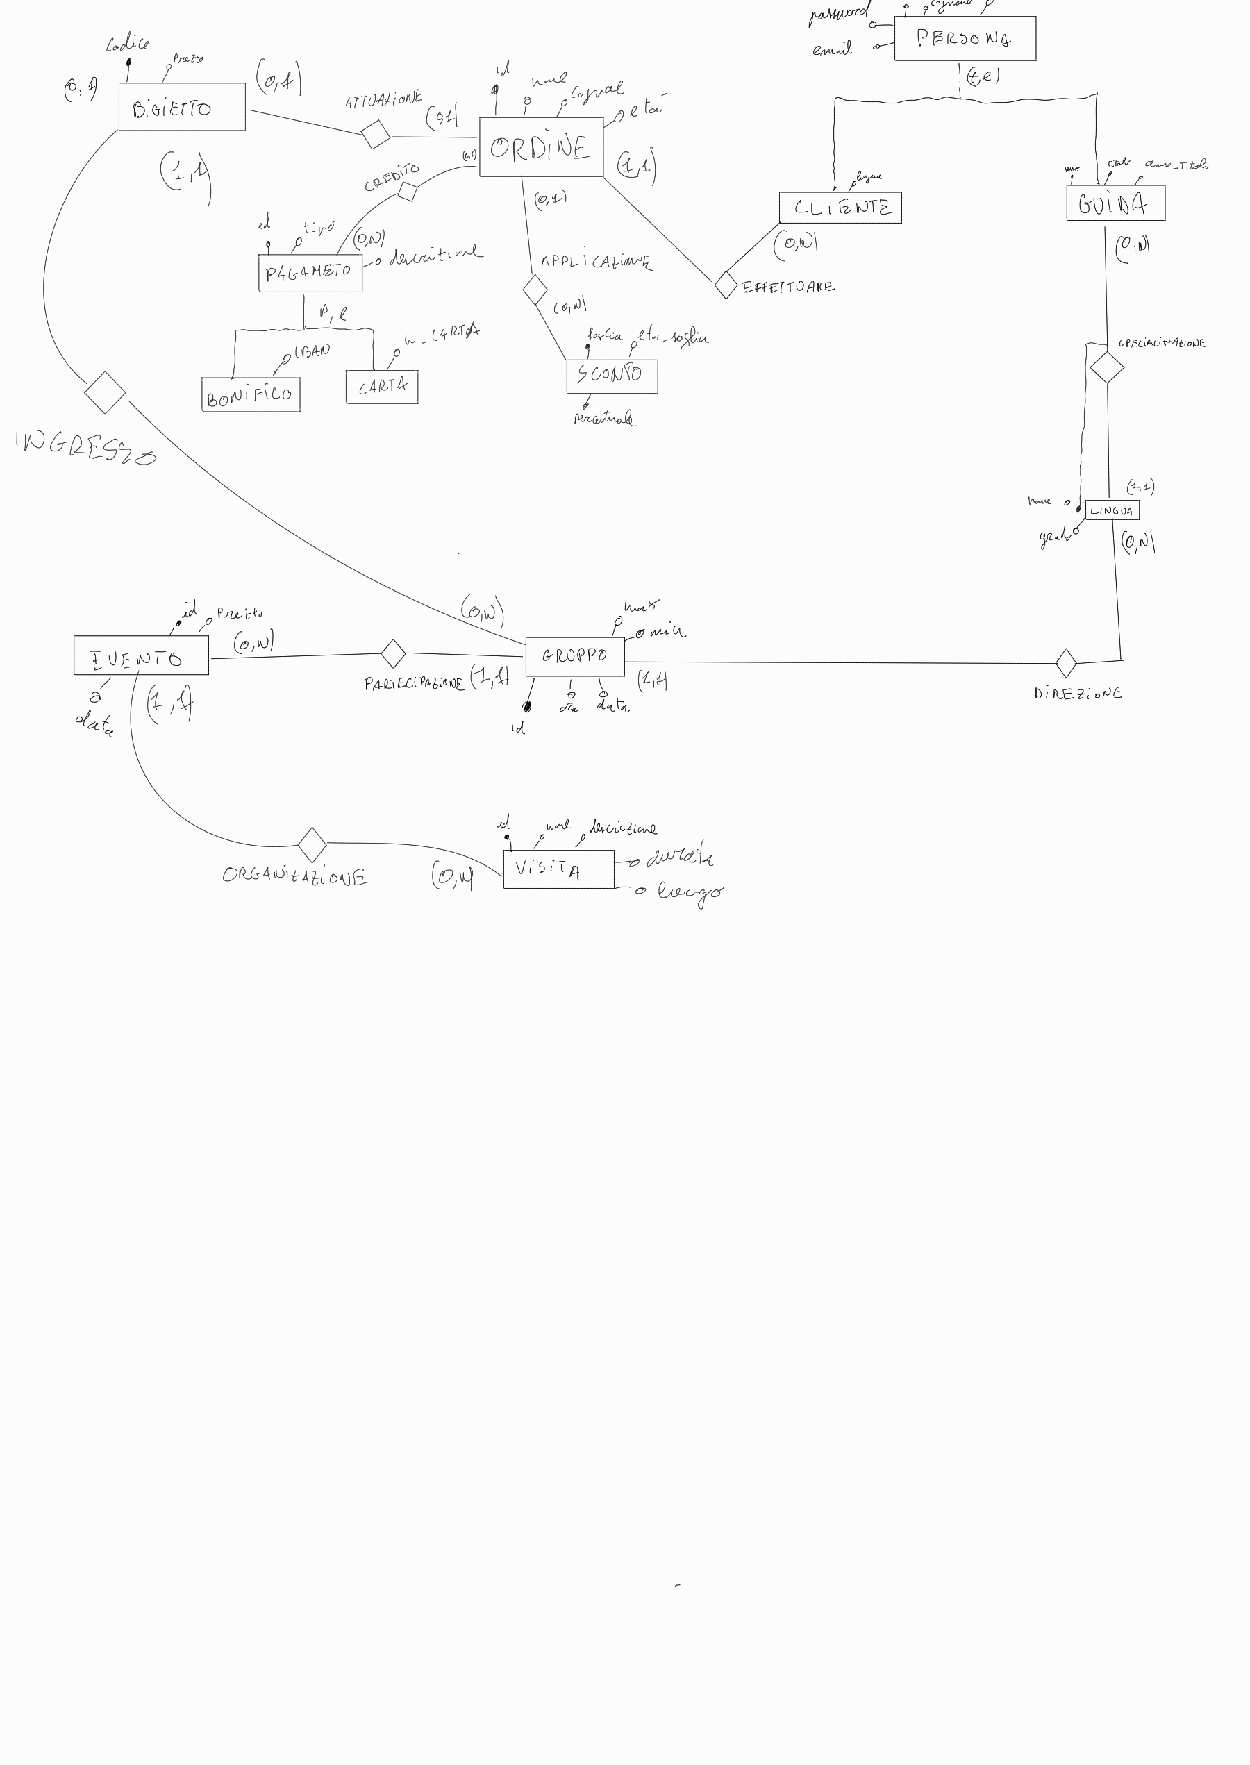
\includepdf[pages=1]{./resources/pdf/ER_turismo.pdf}
\section{Raffinamenti proposti}
\section{Schema concettuale finale}

\newpage
\chapter{Progettazione logica}
\section{Stima del volume dei dati}
\section{Descrizione delle operazioni principali e stima della loro frequenza}
\section{Schemi di navigazione e tabelle degli accessi}
\section{Raffinamento dello schema}
\section{Analisi delle ridondanze}
\section{Traduzione di entità e associazioni in relazioni}


\section{Schema relazionale finale}
\newpage
\section{Traduzione delle operazioni in query SQL}
\begin{lstlisting}[style=codeStyle,language=SQL]
	CREATE TABLE `competenze` (
  	`id_guida` int(11) NOT NULL,
  	`lingua` varchar(15) NOT NULL,
  	`livello` varchar(15) DEFAULT NULL
) ENGINE=InnoDB DEFAULT CHARSET=utf8mb4 COLLATE=utf8mb4_general_ci;
\end{lstlisting}
\newpage
\chapter{Progettazione dell'applicazione}
\end{document}
